%\section{$S_{2}(P)$とコンパクト性}
%\section{正規パターン集合のコンパクト性}
\section{Compactness of Sets of Regular Patterns}

%この節では,コンパクト性の定義を与え,$\sharp\Sigma \ge 2k-1$と仮定したとき,
%$S_{2}(P)$は$\RPatL^{k}$における$L(P)$の特徴集合であることを示し,$\RPat^{k}$が包含に関してコンパクト性を持つことを示す.
In this section, we define the compactness of sets of regular patterns, formally.
Then, if $\sharp\Sigma \ge 2k-1$ holds, 
we show that 
%$S_{2}(P)$ is a character set of $L(P)$ on $\RPatL^{k}$
$\RPat^{k}$ has the compactness with respect to the inclusion property.

\begin{dfn}
%クラス$\mathcal{C} \subseteq \RPatplus$が\textbf{包含に関してコンパクト性を持つ}とは,
%任意のパターン$p \in \RPat$と任意のパターン集合$Q \in \mathcal{C}$に対して,
%$L(p) \subseteq L(Q)$ならば,ある$q \in Q$が存在して$L(p) \subseteq L(q)$であるときをいう.
Let $\mathcal{C}$ be a subset of $\RPatplus$ (resp. $\Patplus$). 
For any regular pattern $p \in \RPat$ (resp. $\Pat$) and any set $Q \in \mathcal{C}$,
the set $\mathcal{C}$ has compactness with respect to inclusion property.
\end{dfn}
%\begin{comment}
%同様にして,クラス$\mathcal{C} \in \Patplus$が包含に関してコンパクト性を持つことが定義できる.
%また,クラス$\mathcal{C} \in \RPatplus$が包含に関してコンパクト性を持つとき,補題\ref{補題1}より,任意の$P, Q \in \mathcal{C}$に対して,$P \sqsubseteq Q$ならばその時に限り$L(P) \subseteq L(Q)$であることが示せる.

\begin{lem}[Sato et al.\cite{Sato1}]\label{変数2つ}
%$\sharp \Sigma \ge 3$とし,$p,~q$を正規パターンとする.
Let $\Sigma$ be an alphabet with $\Sigma \ge 3$ and $p,q$ regular patterns on $\Sigma$.
%正規パターンの有限集合$D$が,次の{\rm (i), (ii)}のいずれかで表されるとき,任意の$r \in D$に対して$p \{ x := r \} \preceq q$ならば,$p \{ x := xy \} \preceq q$である.
%ただし,$a \ne b$とする.
Let $D$ be the set of either $(\mathrm{i})$ or $(\mathrm{ii})$ of regular patterns on $\Sigma$ below: Assume that $a \not= b$ and that a variable symbol $y$ does not appear in $p$.
%\[
\begin{align*}
(\mathrm{i})~~\{ ay, by \}~~~(\mathrm{ii})~\{ ya, yb \}.
\end{align*}
%\]
Then, if $p \{ x := r \} \preceq q$ for all $r \in D$, then $p \{ x := xy \} \preceq q$.
\end{lem}
\begin{proof}
%$p$に変数記号が含まれない場合は自明である.
It is obvious if no variable symbol appears in $p$. 
%したがって,正規パターン$p$には変数記号が現れるとし,その変数記号を$x$とする.
%このとき,正規パターン$p_{1},p_{2}$が存在し,$p=p_{1}xp_{2}$と表すことができる.$p \{ x := xy \} \not \preceq q$と仮定して,矛盾を導く.
Therefore, let $p=p_{1}xp_{2}$, where $p_{1}, p_{2}$ are regular patterns and $x$ is a variable symbol.
We assume that $p \{ x := xy \} \not \preceq q$ in order to derive the contradictions.

\noindent
(i) 
%$D=\{ ay, by \} \ (a \ne b)$であるとする.
The case of $D=\{ ay, by \} \ (a \ne b)$.
%$p \{ x := xy \} \not \preceq q$のとき,$p_{1}ayp_{2}\preceq q$かつ$p_{1}byp_{2}\preceq q$であることから,正規パターン$q_{1},q_{2}$と変数記号$y_{1},y_{2}$,さらに定数記号列$w$が存在して,$q=q_{1}ay_{1}wby_{2}q_{2}$または$q=q_{1}by_{1}way_{2}q_{2}$と表すことができる.
\noindent
Since $p \{ x := xy \} \not \preceq q$, $p_{1}ayp_{2}\preceq q$ and $p_{1}byp_{2}\preceq q$, 
there exist regular patterns $q_{1},q_{2}$ on $\Sigma$ such that $q=q_{1}ay_{1}wby_{2}q_{2}$ or $q=q_{1}by_{1}way_{2}q_{2}$ for some variable symbols $y_{1},y_{2}~(y_{1} \not= y_{2})$ and a constant sequence $w$ ($|w|\geq 0$) from Theorem \ref{Sato1:Lemma9}.
%$q=q_{1}ay_{1}wby_{2}q_{2}$と表されるとき,次の(1), (2), (1'), (2')がすべて成り立つ.
When $q=q_{1}ay_{1}wby_{2}q_{2}$ holds, the following four equations (1), (2), (1'), (2') holds:
\begin{align*}
(1) & ~p_{1} \preceq q_{1}\\
(1') & ~p_{2} \preceq wby_{2}q_{2} \mbox{ or } p_{2} \preceq y^{\prime}wby_{2}q_{2} ~~(y^{\prime} \in X)\\
(2) & ~p_{1} \preceq q_{1}ay_{1}w\\
(2') & ~p_{2} \preceq q_{2} \mbox{ or } p_{2} \preceq y^{\prime\prime}q_{2} ~(y^{\prime\prime} \in X)
\end{align*}
%(2)より,正規パターン$p_{1}^{\prime},p_{1}^{\prime\prime}$が存在して,
%$p_{1}=p_{1}^{\prime}p_{1}^{\prime\prime}$,$p_{1}^{\prime} \preceq q_{1}a$かつ$p_{1}^{\prime\prime} \preceq y_{1}w$
%が成り立つ.
From the above equation (2), there exist regular patterns $p_{1}^{\prime},p_{1}^{\prime\prime}$ such that $p_{1}=p_{1}^{\prime}p_{1}^{\prime\prime}$,$p_{1}^{\prime} \preceq q_{1}a$ and $p_{1}^{\prime\prime} \preceq y_{1}w$ hold.
%したがって,
%$p=p_{1}xp_{2}=p_{1}^{\prime}p_{1}^{\prime\prime}xp_{2}$であるから,
%(1')が$p_{2} \preceq wby_{2}q_{2}$のとき,
%$p\preceq q_{1}ap_{1}^{\prime\prime}xwby_{2}q_{2}=q \{ y_{1} := p_{1}^{\prime\prime}x \}$となる.
Therefore, since $p=p_{1}xp_{2}=p_{1}^{\prime}p_{1}^{\prime\prime}xp_{2}$,
if $p_{2} \preceq wby_{2}q_{2}$ holds, 
$p\preceq q_{1}ap_{1}^{\prime\prime}xwby_{2}q_{2}=q \{ y_{1} := p_{1}^{\prime\prime}x \}$ holds.
%また,(1')が$p_2\preceq y'wby_{2}q_{2}$のとき,$p\preceq q_{1}ap_{1}^{\prime\prime}xy'wby_{2}q_{2}=q \{ y_{1} := p_{1}^{\prime\prime}xy' \}$となる.
Otherwise, that is $p_2\preceq y'wby_{2}q_{2}$, $p\preceq q_{1}ap_{1}^{\prime\prime}xy'wby_{2}q_{2}=q \{ y_{1} := p_{1}^{\prime\prime}xy' \}$ holds.
%よって,$p \preceq q$が成り立ち,
Hence, $p \preceq q$ holds.
%仮定$p \{ x := xy \} \not\preceq q$に矛盾する.
This contradicts the assumption.

\noindent
(ii) 
%\textbf{(ii)} $D=\{ ya, yb \} \ (a \ne b)$のとき
The case of $D=\{ ya, yb \} \ (a \ne b)$.
%は,記号列$p$と$q$を逆順にすることにより,\textbf{(i)}の場合と同様に, 仮定$p \{ x := xy \} \not\preceq q$に矛盾することを証明できる.
By reversing the sequences of $p$ and $q$, we can prove that $p \{ x := xy \} \preceq q$ holds, in a similar way as (i).
\end{proof}

\begin{lem}\label{補題14}
%$\sharp \Sigma \ge 4$とし,$p, q$を正規パターンとする.
%Let $\Sigma$ be an alphabet with $\Sigma \ge 4$ and $p,q$ regular patterns on $\Sigma$.
Let $\Sigma$ be an alphabet with $\Sigma \ge 4$, $p,q$ regular patterns on $\Sigma$.
%正規パターンの有限集合$D= \{ a_{1}b_{1}, a_{2}b_{2}, a_{3}b_{3}, a_{4}b_{4} \}$ $(i \ne j $に対して,$a_{i} \ne a_{j}$かつ$b_{i} \ne b_{j})$で表されるとき,任意の$r \in D$に対して$p \{ x := r \} \preceq q$ならば,$p \{ x := xy \} \preceq q$である.
Let $D$ be the following set of constant sequences on $\Sigma$ whose lengths are just 2:

\medskip
\noindent
~~\begin{tabular}{l}
  $D = \{ a_{1}b_{1}, a_{2}b_{2}, a_{3}b_{3}, a_{4}b_{4} \}$\\
  $(a_{i} \ne a_{j} \mbox{ and } b_{i} \ne b_{j} \mbox{ for each } i,j~(i\ne j, 1\ge i,j\ge 4))$.
\end{tabular}
\medskip

\noindent
We assume that a variable symbol $y$ does not appear in $p$.
Then, if $p \{ x := r \} \preceq q$ for all $r \in D$, then $p \{ x := xy \} \preceq q$.  
\end{lem}
\begin{proof}
%$p$に変数記号が含まれない場合は自明である.
%したがって,正規パターン$p$には変数記号が現れるとし,その変数記号を$x$とする.
%このとき,正規パターン$p_{1},p_{2}$が存在し,$p=p_{1}xp_{2}$と表すことができる.
%$p \{ x := xy \} \not \preceq q$と仮定して,矛盾を導く.
It is obvious if the variable symbol $x$ does not appear in $p$.
Therefore, let $p=p_{1}xp_{2}$, where $p_{1}, p_{2}$ are regular patterns.
We assume that $p \{ x := xy \} \not \preceq q$ in order to derive the contradictions.
%$D=\{ a_{1}b_{1}, a_{2}b_{2}, a_{3}b_{3}, a_{4}b_{4} \}$ $(i \ne j$に対して,$a_{i} \ne a_{j}$かつ$b_{i} \ne b_{j})$であるとする.
%任意の$r \in D$に対して$p \{ x := r \} \preceq q$であることから,
%正規パターン$q$には,$a_{1}b_{1}, a_{2}b_{2}, a_{3}b_{3}, a_{4}b_{4}$に対応する長さ2の記号列が存在する.
Since $p \{ x := r \} \preceq q$ holds for any $r \in D$,
the regular pattern $q$ contains $a_{1}b_{1}, a_{2}b_{2}, a_{3}b_{3}$, and $a_{4}b_{4}$.
%その4つの記号列は一部を重複して現れることがあることに注意する.
We remark that $a_i$ and $b_j$ may be same for $i,j (1\le i,j\le 4)$.
%$D$の4つの記号列に対応する$q$の記号列の現れ方には次の15通り存在する.
Since $p \{ x := r \} \preceq q$ for all $r \in D$ holds, 
there exist the following 15 cases (i)--(xv) for four regular patterns on $\Sigma$ contained in $q$ that correspond to four constant sequences in $D$:
Here, $y_1,y_2,y_3,y_4$ are variable symbols.
%\[

\medskip  
\noindent
\begin{tabular}{ll}
(i)~~~~$a_{1}b_{1}, a_{2}b_{2}, a_{3}b_{3}, a_{4}b_{4}$  & (ix)~~~ $a_{1}b_{1}, y_{1}b_{2}, a_{3}y_{2}, a_{4}y_{3}$ \\
(ii)~~~$a_{1}b_{1}, a_{2}b_{2}, a_{3}b_{3}, a_{4}y_{1}$  & (x)~~~~ $a_{1}b_{1}, a_{2}y_{1}, a_{3}y_{2}, a_{4}y_{3}$ \\
(iii)~~$a_{1}b_{1}, a_{2}b_{2}, a_{3}b_{3}, y_{1}b_{4}$ & (xi)~~~ $y_{1}b_{1}, y_{2}b_{2}, y_{3}b_{3}, y_{4}b_{4}$ \\
(iv)~~~$a_{1}b_{1}, a_{2}b_{2}, a_{3}y_{1}, y_{2}b_{4}$  & (xii)~~ $y_{1}b_{1}, y_{2}b_{2}, y_{3}b_{3}, a_{4}y_{4}$ \\
(v)~~~~$a_{1}b_{1}, a_{2}b_{2}, y_{1}b_{3}, y_{2}b_{4}$    & (xiii)~ $y_{1}b_{1}, y_{2}b_{2}, a_{3}y_{3}, a_{4}y_{4}$ \\
(vi)~~~$a_{1}b_{1}, a_{2}b_{2}, a_{3}y_{1}, a_{4}y_{2}$   & (xiv)~~$y_{1}b_{1}, a_{2}y_{2}, a_{3}y_{3}, a_{4}y_{4}$ \\
(vii)~~$a_{1}b_{1}, y_{1}b_{2}, y_{2}b_{3}, y_{3}b_{4}$  & (xv)~~~$a_{1}y_{1}, a_{2}y_{2}, a_{3}y_{3}, a_{4}y_{4}$ \\
(viii)~$a_{1}b_{1}, y_{1}b_{2}, y_{2}b_{3}, a_{4}y_{3}$ &        %& ($y_{1},y_{2},y_{3},y_{4}$は変数記号)
\end{tabular}
%\]
\medskip

%上記\textbf{(e)--(o)}の11通りの記号列を含む正規パターン$q$は,
%補題\ref{変数2つ}(i)または(ii)に対応する記号列が現れる.
\noindent
For the cases (v)--(xv), we can prove that $p \{ x := xy \} \preceq q$ holds in a similar way as Lemma \ref{変数2つ}.
%その場合の証明より仮定$p \{ x := xy \} \not\preceq q$に矛盾する.
%したがって,(a)--(d)の4通りついて矛盾を導く.
Hence, for the cases (i)--(iv), we will prove that $p \{ x := xy \} \preceq q$ holds.

%(a), (b), (c)は,$q$に$a_{1}b_{1}, a_{2}b_{2}, a_{3}b_{3}, a_{4}b_{4}$が現れる場合,(d)は, $q$に$a_{1}b_{1}, a_{2}b_{2}, a_{3}y_{1}, y_{2}b_{4}$が現れる場合において,矛盾を導く証明が考えられる.
%しかし,(a), (b), (c)は,$q$に$a_{1}b_{1}, a_{2}b_{2}, a_{3}b_{3}$が現れる場合,(d)は, $q$に$a_{1}b_{1}, a_{2}b_{2}, a_{3}y_{1}$が現れる場合と$q$に$a_{1}b_{1}, a_{2}b_{2}, y_{2}b_{4}$が現れる場合において,矛盾を導くことで,証明できる.
%よって,本論文では,$q$に$a_{1}b_{1}, a_{2}b_{2}, a_{3}b_{3}$が現れる場合と$q$に$a_{1}b_{1}, a_{2}b_{2}, a_{3}y$ $(y=y_{1})$が現れる場合を証明する.
%$q$に$a_{1}b_{1}, a_{2}b_{2}, y_{2}b_{4}$が現れる場合は,記号列$p$と$q$を逆順にすることにより,$q$に$a_{1}b_{1}, a_{2}b_{2}, a_{3}y$が現れる場合の証明から導かれる.
%\smallskip

\smallskip
\noindent
%\textbf{(abc)} $q$に$a_{1}b_{1}, a_{2}b_{2}, a_{3}b_{3}$が現れる場合,
(I) Cases of (i), (ii) and (iii), that is the cases that $q$ contains $a_{1}b_{1}, a_{2}b_{2}$ and $a_{3}b_{3}$:

%\begin{figure}[H]
\begin{figure}
\centering
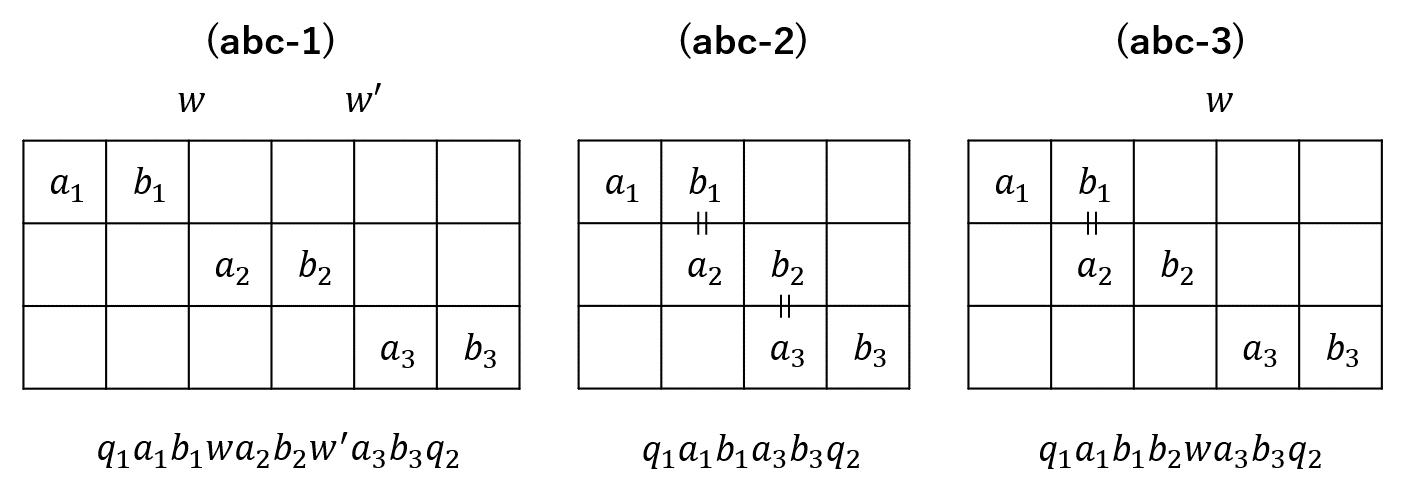
\includegraphics[width=\linewidth]{figs/Cases-abc.png}
\vspace{-1cm}
\caption{(abc)の場合分け}
\label{abc組み合わせ}
\end{figure}

%図\ref{abc組み合わせ}のように,3つの記号列が重複する場合があるので,次の3つの場合に分けて証明する.
\noindent
We consider the following three cases (I-1)-(I-3) of $q$ for some regular patterns $q_{1},q_{2}$ and some constant sequences $w,w^{\prime}$ ($|w|\geq 0$ and $|w^{\prime}|\geq 0$):
\[
\begin{tabular}{ll}
(I-1) $q=q_{1}a_{1}b_{1}wa_{2}b_{2}w^{\prime}a_{3}b_{3}q_{2}$,\\
(I-2) $q=q_{1}a_{1}b_{1}a_{3}b_{3}q_{2}$ ($b_{1}=a_{2}$ and $a_{3}=b_{2}$),\\
(I-3) $q=q_{1}a_{1}b_{1}b_{2}wa_{3}b_{3}q_{2}$ ($b_{1}=a_{2}$)\\
(I-4) $q=q_{1}a_{1}b_{1}wa_{2}b_{2}b_{3}q_{2}$ ($b_{2}=a_{3}$).
\end{tabular}
\]

%\textbf{(abc-1)} $q=q_{1}a_{1}b_{1}wa_{2}b_{2}w^{\prime}a_{3}b_{3}q_{2}$とする.これに対して,次の式が成り立っているものとする.
\noindent
(I-1) Case of $q=q_{1}a_{1}b_{1}wa_{2}b_{2}w^{\prime}a_{3}b_{3}q_{2}$:
Assume that the following six equations (1),(2),(3),(1'),(2'),(3') are hold.
\begin{align*}
(1)~& p_{1} \preceq q_{1} & (\text{1'})~& p_{2} \preceq wa_{2}b_{2}w^{\prime}a_{3}b_{3}q_{2} \\
(2)~& p_{1} \preceq q_{1}a_{1}b_{1}w & (\text{2'})~& p_{2} \preceq w^{\prime}a_{3}b_{3}q_{2} \\
(3)~& p_{1} \preceq q_{1}a_{1}b_{1}wa_{2}b_{2}w^{\prime} & (\text{3'})~& p_{2} \preceq q_{2}
\end{align*}

%$|w|=|w^{\prime}|$のとき,(2)と(3)より,$p_{1}$の接尾辞は$a_{1}b_{1}wa_{2}b_{2}w^{\prime}$かつ$a_{1}b_{1}w$であるので,$a_{1}b_{1}w=a_{2}b_{2}w^{\prime}$となる.よって,$a_{1}b_{1}=a_{2}b_{2}$となり,$a_{1} \ne a_{2}$かつ$b_{1} \ne b_{2}$であることに矛盾する.
If $|w|=|w^{\prime}|$ holds, $a_{1}b_{1}wa_{2}b_{2}w^{\prime}$ and $a_{1}b_{1}w$ are the suffix of $p_{1}$ from the above equations (2) and (3).
Then, $a_{1}b_{1}w=a_{2}b_{2}w^{\prime}$.
Hence, $a_{1}b_{1}=a_{2}b_{2}$.
This contracts the assumption of $a_{1} \ne a_{2}$ and $b_{1} \ne b_{2}$.

%$|w|+1=|w^{\prime}|$のとき,(1')と(2')より,$p_{2}$の接頭辞は$wa_{2}b_{2}w^{\prime}a_{3}b_{3}$かつ$w^{\prime}a_{3}b_{3}$である.
If $|w|+1=|w^{\prime}|$ holds, $wa_{2}b_{2}w^{\prime}a_{3}b_{3}$ and $w^{\prime}a_{3}b_{3}$ are the prefix of $p_{2}$.
%$w^{\prime}=ww_{1}$とおくと,$w^{\prime}a_{3}b_{3}=ww_{1}a_{3}b_{3}$となる.
If there exists a constant symbol $w_{1}$ such that $w^{\prime}a_{3}b_{3}=ww_{1}a_{3}b_{3}$,
%したがって,$wa_{2}b_{2}=ww_{1}a_{3}$より$b_{2}=a_{3}$となる.
then $b_{2}$ and $a_{3}$ are the same symbol from $wa_{2}b_{2}=ww_{1}a_{3}$.
%(2)と(3)より,$p_{1}$の接尾辞は$a_{1}b_{1}wa_{2}b_{2}w^{\prime}, a_{1}b_{1}w$である.
From the above equations (2) and (3), $a_{1}b_{1}wa_{2}b_{2}w^{\prime}$ and $a_{1}b_{1}w$ are the suffix of $p_{1}$.
%$w^{\prime}=w_{2}w$とおくと,$a_{1}b_{1}wa_{2}b_{2}w^{\prime}=a_{1}b_{1}wa_{2}b_{2}w_{2}w$となる.
Then, there exists a constant symbol $w_{2}$ such that $w^{\prime}=w_{2}w$,
%したがって,$b_{2}w_{2}w=a_{1}b_{1}w$より,$b_{2}=a_{1}$となる.
then $b_{2}$ and $a_{1}$ are the same symbol from $b_{2}w_{2}w=a_{1}b_{1}w$.
Hence, from $b_{2}=a_{3}$, $a_{3}$ and $a_{1}$ are same symbol.
This contradicts the assumption of $a_{3} \ne a_{1}$.

%$|w|+1 < |w^{\prime}|$のとき,(2)と(3)より,$p_{1}$の接尾辞は$a_{1}b_{1}wa_{2}b_{2}w^{\prime}$かつ$a_{1}b_{1}w$である.
If $|w|+1 < |w^{\prime}|$, from the above (2) and (3), 
$a_{1}b_{1}wa_{2}b_{2}w^{\prime}$ and $a_{1}b_{1}w$ are the suffix of $p_{1}$.
%$w^{\prime}=w_{1}w$とおくと,$a_{1}b_{1}wa_{2}b_{2}w^{\prime}=a_{1}b_{1}wa_{2}b_{2}w_{1}w$となる.
If there exists a constant sequence $w_{1}$ ($|w_{1}|\geq 2$) such that $w^{\prime}=w_{1}w$, then $a_{2}b_{2}$ is the suffix of $w_{1}$.
%$|w_{1}| \ge 2$であるため,$w_{1}$の接尾辞は$a_{2}b_{2}$となる.
%
%($1'$)と($2'$)より,$p_{2}$の接頭辞は$wa_{2}b_{2}w^{\prime}a_{3}b_{3}$かつ$w^{\prime}a_{3}b_{3}$である.
From  the above equations ($1'$) and ($2'$), 
$wa_{2}b_{2}w^{\prime}a_{3}b_{3}$ and $w^{\prime}a_{3}b_{3}$ are the prefix of $p_{2}$.
%$w^{\prime}=ww_{2}$とおくと,$w^{\prime}a_{3}b_{3}=ww_{2}a_{3}b_{3}$となり,$w^{\prime}=w_{1}w$とおくと,$wa_{2}b_{2}w^{\prime}a_{3}b_{3}=wa_{2}b_{2}w_{1}wa_{3}b_{3}$となる.
%$|ww_{2}a_{3}b_{3}|=|wa_{2}b_{2}w_{1}|$より,$w_{1}$の接尾辞は$a_{3}b_{3}$となる.
If there exist constant sequences $w_{1}$ and $w_{2}$ such that $w^{\prime} = w_{1}w=ww_{2}$ holds, then $a_{2}b_{2}$ and $a_{3}b_{3}$ are the suffix of $w_{1}$ from $|ww_{2}a_{3}b_{3}|=|wa_{2}b_{2}w_{1}|$.
%よって,$w_{1}$の接尾辞は$a_{2}b_{2}=a_{3}b_{3}$となり,$a_{2} \ne a_{3}$かつ$b_{2} \ne b_{3}$であることに矛盾する.
Hence, $a_{2}b_{2}=a_{3}b_{3}$.
This contradicts the assumption of $a_{2} \ne a_{3}$ and $b_{2} \ne b_{3}$.
\smallskip

%\textbf{(abc-2)} $q=q_{1}a_{1}b_{1}a_{3}b_{3}q_{2}$ ($b_{1}=a_{2}$かつ$a_{3}=b_{2}$)とする.
\noindent
(I-2) Case of $q=q_{1}a_{1}b_{1}a_{3}b_{3}q_{2}$ ($b_{1}=a_{2}$ and $a_{3}=b_{2}$):
%これに対して,次の式が成り立っているものとする.
Assume that the following six equations (1),(2),(3),(1'),(2'),(3') are hold.
\begin{align*}
(1)~& p_{1} \preceq q_{1} & (\text{1'})~& p_{2} \preceq a_{3}b_{3}q_{2} \\
(2)~& p_{1} \preceq q_{1}a_{1} & (\text{2'})~& p_{2} \preceq b_{3}q_{2} \\
(3)~& p_{1} \preceq q_{1}a_{1}b_{1} & (\text{3'})~& p_{2} \preceq q_{2}
\end{align*}

\noindent
%(2)と(3)より,$p_{1}$の接尾辞は$a_{1}b_{1}$かつ$a_{1}$であり,$b_{1}=a_{1}$となる.$b_{1}=a_{2}$より,$a_{1}=a_{2}$であるため, $a_{1} \ne a_{2}$であることに矛盾する.
From the above equations (2) and (3), since $a_{1}b_{1}$ and $a_{1}$ are the suffix of $p_{1}$, 
$b_{1} = a_{1}$ holds.
From the assumption of $b_{1}=a_{2}$, $a_{1}=a_{2}$.
This contradicts the assumption of $a_{1}\not= a_{2}$.
\smallskip

\noindent
%\textbf{(abc-3)} $q=q_{1}a_{1}b_{1}b_{2}wa_{3}b_{3}q_{2}$ ($b_{1}=a_{2}$)とする.これに対して,次の式が成り立っているものとする.
(I-3) Case of $q=q_{1}a_{1}b_{1}b_{2}wa_{3}b_{3}q_{2}$ ($b_{1}=a_{2}$):
%これに対して,次の式が成り立っているものとする.
Assume that the following six equations (1),(2),(3),(1'),(2'),(3') are hold.
\begin{align*}
(1)~& p_{1} \preceq q_{1} & (\text{1'})~& p_{2} \preceq b_{2}wa_{3}b_{3}q_{2} \\
(2)~& p_{1} \preceq q_{1}a_{1} & (\text{2'})~& p_{2} \preceq wa_{3}b_{3}q_{2} \\
(3)~& p_{1} \preceq q_{1}a_{1}b_{1}b_{2}w & (\text{3'})~& p_{2} \preceq q_{2}
\end{align*}
\noindent
%$w=\varepsilon$のとき,(2)と(3)より,$p_{1}$の接尾辞は$a_{1}$かつ$a_{1}b_{1}b_{2}$であり,(1')と(2')より,$p_{2}$の接頭辞は$b_{2}a_{3}b_{3}$かつ$a_{3}b_{3}$である.
If $|w|=0$, that is $w=\varepsilon$, then $a_{1}$ and $a_{1}b_{1}b_{2}$ are the suffix of $p_{1}$ from the above equations (2) and (3)
and $b_{2}a_{3}b_{3}$ and $a_{3}b_{3}$ are the prefix of $p_{2}$ from the above equations (1') and (2').
%$b_{2}=a_{1}$と$b_{2}a_{3}=a_{3}b_{3}$より,$a_{1}=a_{3}$となり,$a_{1} \ne a_{3}$であることに矛盾する.
Since $b_{2}=a_{1}$ and $b_{2}a_{3}=a_{3}b_{3}$, $a_{1}=a_{3}$ holds.
This contradicts the assumption of $a_{1}\not= a_{3}$.

%$|w| \ge 1$のとき,(2)と(3)より,$p_{1}$の接尾辞は$a_{1}$かつ$a_{1}b_{1}b_{2}w$である.
\noindent
If $|w| \ge 1$, $a_{1}$ and $a_{1}b_{1}b_{2}w$ are the suffix of $p_{1}$ from the above equations (2) and (3).
%よって,$w$の最後の記号は$a_{1}$となる.
Hence, the last symbol of $w$ is $a_{1}$.
%(1')と(2')より,$p_{2}$の接頭辞は$b_{2}wa_{3}b_{3}$かつ$wa_{3}b_{3}$となる.
Moreover, $b_{2}wa_{3}b_{3}$ and $wa_{3}b_{3}$ are the prefix of $p_{2}$ from the above equations (1') and (2').
%よって,$w$の最後の記号は$a_{3}$となる.
Hence, the last symbol of $w$ is $a_{3}$.
%したがって,$w$の最後の記号は$a_{1}=a_{3}$となり,$a_{1} \ne a_{3}$であることに矛盾する.
Therefore, $a_{1}=a_{3}$ holds.
This contradicts the assumption of $a_{1} \ne a_{3}$.
\smallskip

\noindent
%\textbf{(d)} $q$に$a_{1}b_{1}, a_{2}b_{2}, a_{3}y$が現れる場合,記号列$A,B,C$に対して,$\{ A, B, C \} = \{ a_{1}b_{1}, a_{2}b_{2}, a_{3}y \}$とおき,$q=q_{1}AwBw^{\prime}Cq_{2}$とする.
(II) Case of (iv), that is, $q$ contains $a_{1}b_{1}, a_{2}b_{2}$ and $a_{3}y$:
%これに対して,次の式が成り立っているものとする.
Let $A,B,C$ be distinct regular patterns in $\{a_{1}b_{1}, a_{2}b_{2}, a_{3}y\}$ such that $q=q_{1}AwBw^{\prime}Cq_{2}$.
Assume that the following six equations (1),(2),(3),(1'),(2'),(3') are hold.
\begin{align*}
(1)~& p_{1} \preceq q_{1} & (\text{1'})~& p_{2} \preceq wBw^{\prime}Cq_{2} \\
(2)~& p_{1} \preceq q_{1}Aw & (\text{2'})~& p_{2} \preceq w^{\prime}Cq_{2} \\
(3)~& p_{1} \preceq q_{1}AwBw^{\prime} & (\text{3'})~& p_{2} \preceq q_{2}
\end{align*}

\noindent
%$|w|=|w^{\prime}|$のとき,(2)と(3)より,$p_{1}$の接尾辞は$Aw$かつ$AwBw^{\prime}$である.
If $|w|=|w^{\prime}|$, then $Aw$ and $AwBw^{\prime}$ are the suffix of $p_{1}$ from the above equations (2) and (3).
%よって,$Aw=Bw^{\prime}$となり,$A \ne B$であることに矛盾する.
Hence, $Aw=Bw^{\prime}$ holds.
This contradicts the assumption of $A \ne B$.

\noindent
%$|w| \ne |w^{\prime}|$とする.
If $|w| \ne |w^{\prime}|$, then we consider the two cases $A=a_{3}y$ and $B=a_{3}y$:
%$A=a_{3}y$とすると,$B=a_{1}b_{1}$,$C=a_{2}b_{2}$としてよいので,(2)は$p_{1} \preceq q_{1}a_{3}yw$となる.
In the case of $A=a_{3}y$,without losing generality, we assume that $B=a_{1}b_{1}$ and $C=a_{2}b_{2}$. 
%したがって,正規パターン$p_{1}', p_{1}''$が存在して,$p_{1}=p_{1}'p_{1}''$,$p_{1}^{\prime} \preceq q_{1}a_{3}$かつ$p_{1}^{\prime\prime} \preceq yw$となる.
Then, there exist regular patterns $p_{1}^{\prime}, p_{1}^{\prime\prime}$ such that $p_{1}=p_{1}^{\prime}p_{1}^{\prime\prime}$, $p_{1}^{\prime} \preceq q_{1}a_{3}$ and $p_{1}^{\prime\prime} \preceq yw$ from the above equation (2).
%これらと(1')より,$p=p_{1}xp_{2}=p_{1}^{\prime}p_{1}^{\prime\prime}xp_{2}\preceq q_{1}a_{3}p_{1}^{\prime\prime}xwa_{1}b_{1}w^{\prime}a_{2}b_{2}q_{2}=q \{ y := p_{1}^{\prime\prime}x \}$となり,$p=q \theta$となる.
Moreover, from the above equation (1'), $p=p_{1}xp_{2}=p_{1}^{\prime}p_{1}^{\prime\prime}xp_{2}\preceq q_{1}a_{3}p_{1}^{\prime\prime}xwa_{1}b_{1}w^{\prime}a_{2}b_{2}q_{2}=
q_{1}a_{3}ywa_{1}b_{1}w^{\prime}a_{2}b_{2}q_{2}\{ y := p_{1}^{\prime\prime}x \}=q \{ y := p_{1}^{\prime\prime}x \}$ holds.
Hence, $p \preceq q$ holds.
This contracts the assumption.
%これは仮定に矛盾する.
%$B=a_{3}y$とすると,$A=a_{1}b_{1}$,$C=a_{2}b_{2}$としてよいので,(3)は$p_{1} \preceq q_{1}a_{1}b_{1}wa_{3}yw^{\prime}$となり,(1')は$p_{2} \preceq wa_{3}yw^{\prime}a_{2}b_{2}q_{2}$である.$q_{1}^{\prime}=q_{1}a_{1}b_{1}$,$q_{2}^{\prime}=wa_{3}yw^{\prime}$,$q_{3}^{\prime}=a_{2}b_{2}q_{2}$とおくと, (3)~$p_{1} \preceq q_{1}^{\prime}q_{2}^{\prime}, (1')~p_{2} \preceq q_{2}^{\prime}q_{3}^{\prime}, q_{2}^{\prime}$は変数記号が含まれる.
In the case of $B=a_{3}y$, without losing generality, we assume that $A=a_{1}b_{1}$ and $C=a_{2}b_{2}$.
%(3)は$p_{1} \preceq q_{1}a_{1}b_{1}wa_{3}yw^{\prime}$となり,(1')は$p_{2} \preceq wa_{3}yw^{\prime}a_{2}b_{2}q_{2}$である.
Let $q_{1}^{\prime}=q_{1}a_{1}b_{1}$, $q_{2}^{\prime}=wa_{3}yw^{\prime}$, and $q_{3}^{\prime}=a_{2}b_{2}q_{2}$ such that $q_{2}^{\prime}$ contains at most one variable symbol.
Then, the above equations (3) and (1') are represented by $p_{1} \preceq q_{1}^{\prime}q_{2}^{\prime}$ and $p_{2} \preceq q_{2}^{\prime}q_{3}^{\prime}$, respectively.
%補題\ref{補題9}より,$p \preceq q$となり,$p \{ x := xy \} \preceq q$である.
From Theorem \ref{Sato1:Lemma9}, $p \preceq q$ holds.
This contradicts the assumption.
%これは仮定に矛盾する.


\begin{figure}
  \centering
  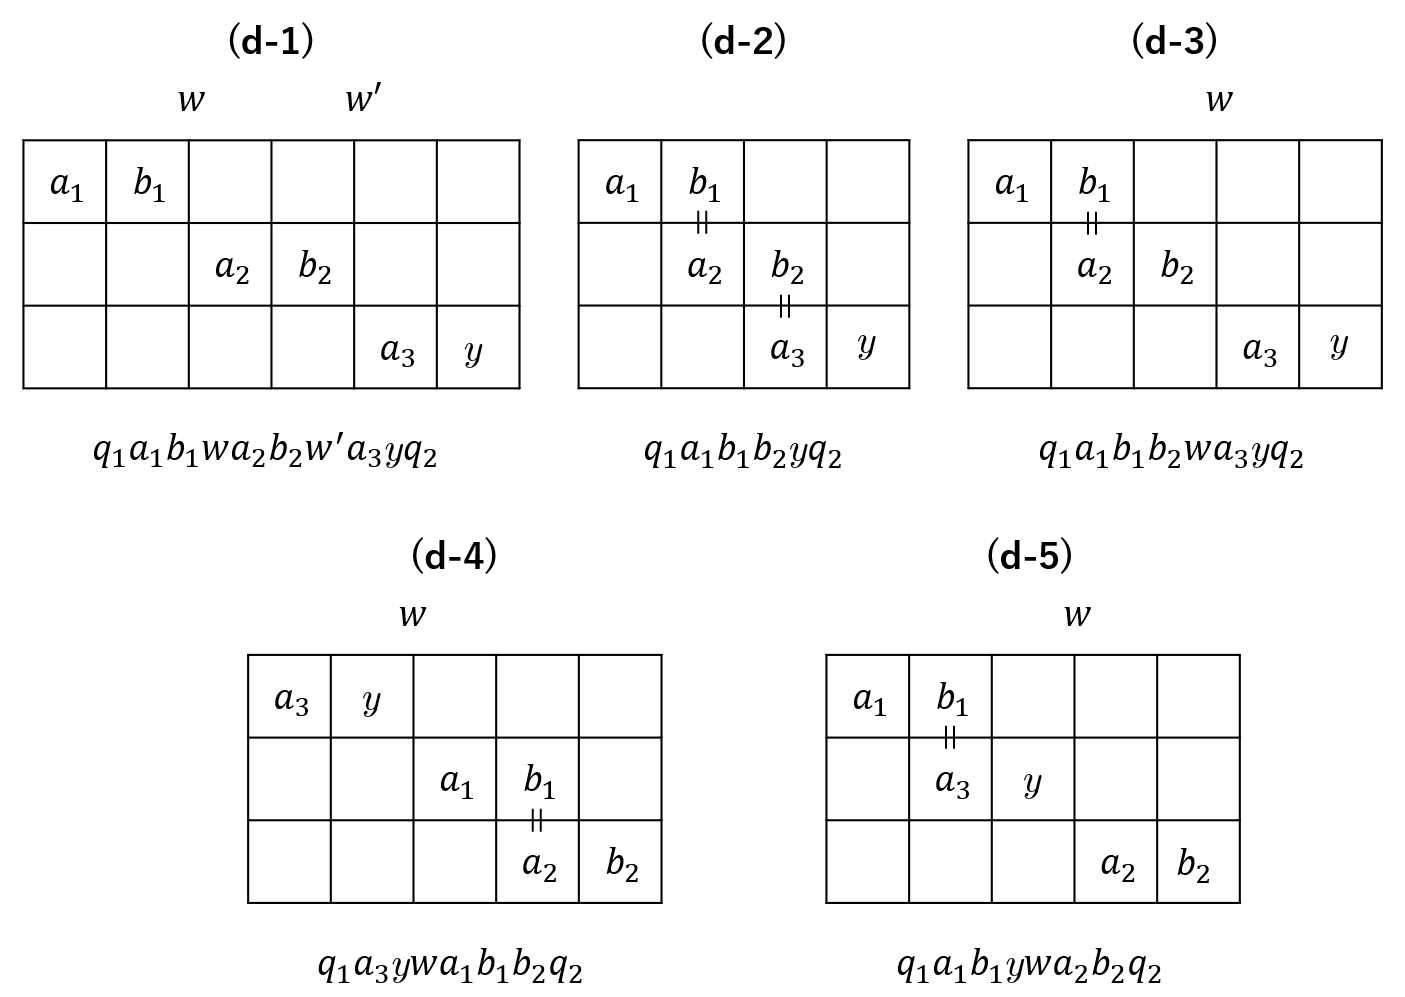
\includegraphics[width=\linewidth]{figs/Cases-d.png}
  \vspace{-1cm}
  \caption{(d)の場合分け}
  \label{d組み合わせ}
\end{figure}
    
%以上より,$A$または$B$が$a_{3}y$の場合,仮定に矛盾するため,$C=a_{3}y$となる.
Next, in the case of $C=a_{3}y$, we consider the following five cases (II-1)--(II-5):
%$C=a_{3}y$のとき,3つの記号列が重複する場合を考慮して,表\ref{d組み合わせ}のように,5つの場合に分けて証明する.
%\[

\begin{tabular}{l}
(II-1) $q=q_{1}a_{1}b_{1}wa_{2}b_{2}w^{\prime}a_{3}yq_{2}$,\\
(II-2) $q=q_{1}a_{1}b_{1}b_{2}yq_{2}$ ($a_{2}=b_{1}$ and $a_{3}=b_{2}$),\\
(II-3) $q=q_{1}a_{1}b_{1}b_{2}wa_{3}yq_{2}$ ($b_{1}=a_{2}$),\\
(II-4) $q=q_{1}a_{3}ywa_{1}b_{1}b_{2}q_{2}$ ($b_{1}=a_{2}$),\\
(II-5) $q=q_{1}a_{1}b_{1}ywa_{2}b_{2}q_{2}$ ($b_{1}=a_{3}$).
\end{tabular}
%\]

\noindent
%\textbf{(d-1)} $q=q_{1}a_{1}b_{1}wa_{2}b_{2}w^{\prime}a_{3}yq_{2}$とする.これに対して,次の式が成り立っているものとする.
(II-1) Case of $q=q_{1}a_{1}b_{1}wa_{2}b_{2}w^{\prime}a_{3}yq_{2}$:
%これに対して,次の式が成り立っているものとする.
Assume that the following six equations (1),(2),(3),(1'),(2'),(3') are hold.
\begin{align*}
(1)~& p_{1} \preceq q_{1} & (\text{1'})~& p_{2} \preceq wa_{2}b_{2}w^{\prime}a_{3}yq_{2} \\
(2)~& p_{1} \preceq q_{1}a_{1}b_{1}w & (\text{2'})~& p_{2} \preceq w^{\prime}a_{3}yq_{2} \\
(3)~& p_{1} \preceq q_{1}a_{1}b_{1}wa_{2}b_{2}w^{\prime} & (\text{3'})~& p_{2} \preceq q_{2}
\end{align*}

\noindent
%$|w|+1=|w^{\prime}|$のとき,(2)と(3)より,$p_{1}$の接尾辞は$a_{1}b_{1}wa_{2}b_{2}w^{\prime}$かつ$a_{1}b_{1}w$である.
If $|w|+1=|w^{\prime}|$, then $a_{1}b_{1}wa_{2}b_{2}w^{\prime}$ and $a_{1}b_{1}w$ are the suffix of $p_{1}$ from the above equations (2) and (3).
%$w^{\prime}=w_{1}w$とおくと,$a_{1}b_{1}wa_{2}b_{2}w^{\prime}=a_{1}b_{1}wa_{2}b_{2}w_{1}w$と表すことができる.
%$b_{2}w_{1}w=a_{1}b_{1}w$より,$b_{2}=a_{1}$となる.
Since there exists a constant symbol $w_{1}$ such that $w^{\prime}=w_{1}w$ and $b_{2}w_{1}w=a_{1}b_{1}w$ hold,
then $b_{2}=a_{1}$.
%(1')と(2')より,$p_{2}$の接頭辞は$wa_{2}b_{2}w^{\prime}a_{3}$かつ$w^{\prime}a_{3}$である.
Moreover, $wa_{2}b_{2}w^{\prime}a_{3}$ and $w^{\prime}a_{3}$ are the prefix of $p_{2}$ from the above equations (1') and (2').
%$w^{\prime}=ww_{2}$とおくと, $w^{\prime}a_{3}=ww_{2}a_{3}$と表すことができる.$wa_{2}b_{2}=ww_{2}a_{3}$より,$b_{2}=a_{3}$となる.
Since there exists a constant symbol $w_{2}$ such that $w^{\prime}=ww_{2}$ and $wa_{2}b_{2}=ww_{2}a_{3}$ hold,
then $b_{2}=a_{3}$.
%よって,$b_{2}=a_{1}$より,$a_{1}=a_{3}$となり,$a_{1} \ne a_{3}$であることに矛盾する.
Thus, $a_{1} = a_{3}$ holds.
This contradicts the assumption of $a_{1} \ne a_{3}$.

\noindent
%$|w|+1 < |w^{\prime}|$のとき,(2)と(3)より,$p_{1}$の接尾辞は$a_{1}b_{1}wa_{2}b_{2}w^{\prime}$かつ$a_{1}b_{1}w$である.
IF $|w|+1 < |w^{\prime}|$, then $a_{1}b_{1}wa_{2}b_{2}w^{\prime}$ and $a_{1}b_{1}w$ are the suffix of $p_{1}$ from the above equations (2) and (3).
Hence, $a_{1}b_{1}$ is the suffix of $w_{\prime}$.
%$w^{\prime}=w_{1}w$とおくと,$a_{1}b_{1}wa_{2}b_{2}w^{\prime}=a_{1}b_{1}wa_{2}b_{2}w_{1}w$と表すことができる.
%よって,$w_{1}$の接尾辞は$a_{1}b_{1}$となる.
%(1')と(2')より,$p_{2}$の接頭辞は$wa_{2}b_{2}w^{\prime}a_{3}$かつ$w^{\prime}a_{3}$である.
Moreover, $wa_{2}b_{2}w^{\prime}a_{3}$ and $w^{\prime}a_{3}$ are the prefix of $p_{2}$ from the above equations (1') and (2').
%$w^{\prime}=w_{1}w$とおくと,$wa_{2}b_{2}w^{\prime}a_{3}=wa_{2}b_{2}w_{1}wa_{3}$となる.
%さらに,$w^{\prime}=ww_{2}$とおくと,$w^{\prime}a_{3}=ww_{2}a_{3}$と表すことができる.$|a_{2}b_{2}w_{1}|=|w_{2}a_{3}|+1$より,$w_{1}$の最後から2つ目の記号は$a_{3}$となる.よって,$w_{1}$の接尾辞は$a_{1}b_{1}$であり,$a_{1}=a_{3}$となる.
Hence, there exist constant symbols $w_{1}$ and $w_{2}$ suth that $w^{\prime}=w_{1}w$, $w^{\prime}=ww_{2}$ and $|a_{2}b_{2}w_{1}|=|w_{2}a_{3}|+1$ hold.
Thus, since the second-to-last symbol of $w_{1}$ is $a_{3}$, $a_{1}=a_{3}$ holds.
%これは,$a_{1} \ne a_{3}$であることに矛盾する.
This contradicts the assumption of $a_{1} \ne a_{3}$.

\noindent
%$|w^{\prime}|+1=|w|$のとき,(1')と(2')より,$p_{2}$の接頭辞は$wa_{2}b_{2}w^{\prime}a_{3}$かつ$w^{\prime}a_{3}$である.
If $|w^{\prime}|+1=|w|$, then $wa_{2}b_{2}w^{\prime}a_{3}$ and $w^{\prime}a_{3}$ are the prefix of $p_{2}$ from the above equations (1') and (2').
%$w=w^{\prime}w_{1}$とおくと,$wa_{2}b_{2}w^{\prime}a_{3}=w^{\prime}w_{1}a_{2}b_{2}w^{\prime}a_{3}$と表すことができる.
%$w^{\prime}w_{1}=w^{\prime}a_{3}$より,$w_{1}=a_{3}$となる.(2)と(3)より,$p_{1}$の接尾辞は$a_{1}b_{1}wa_{2}b_{2}w^{\prime}$かつ$a_{1}b_{1}w$である.
%$w=w^{\prime}w_{1}$とおくと,$a_{1}b_{1}wa_{2}b_{2}w^{\prime}=a_{1}b_{1}w^{\prime}w_{1}a_{2}b_{2}w^{\prime}$となる.
%さらに,$w=w_{2}w^{\prime}$とおくと,$a_{1}b_{1}w=a_{1}b_{1}w_{2}w^{\prime}$と表すことができる.
%$|w_{1}a_{2}b_{2}w^{\prime}|=|a_{1}b_{1}w_{2}w^{\prime}|$より,$w_{1}=a_{1}$となる.よって,$w_{1}=a_{3}$より,$a_{1}=a_{3}$となり,$a_{1} \ne a_{3}$であることに矛盾する.
Since there exists a constant symbol $w_{1}$ such that $w=w^{\prime}w_{1}$ and $w^{\prime}w_{1}=w^{\prime}a_{3}$ hold, then $w_{1}=a_{3}$ holds.
Moreover, since $a_{1}b_{1}wa_{2}b_{2}w^{\prime}$ and $a_{1}b_{1}w$ are the suffix of $p_{1}$ from the above equations (2) and (3), 
there exists a constant symbol $w_{2}$ such that $w=w_{2}w^{\prime}$ and $|w_{1}a_{2}b_{2}w^{\prime}|=|a_{1}b_{1}w_{2}w^{\prime}|$ hold.
Hence, $w_{1}=a_{1}$ holds.
Thus, $a_{1}=a_{3}$ holds.
This contradicts the assumption of $a_{1}\ne a_{3}$.

\noindent
%$|w| > |w^{\prime}|+1$のとき,(1')と(2')より,$p_{2}$の接頭辞は$wa_{2}b_{2}w^{\prime}a_{3}$かつ$w^{\prime}a_{3}$である.
IF $|w| > |w^{\prime}|+1$, since $wa_{2}b_{2}w^{\prime}a_{3}$ and $w^{\prime}a_{3}$ are the prefix of $p_{2}$ from the above equations (1') and (2'),
%$w=w^{\prime}w_{1}$とおくと,$wa_{2}b_{2}w^{\prime}a_{3}=w^{\prime}w_{1}a_{2}b_{2}w^{\prime}a_{3}$と表すことができる.
%このとき,$w_{1}$の最初の記号は$a_{3}$となる.(2)と(3)より,$p_{1}$の接尾辞は$a_{1}b_{1}wa_{2}b_{2}w^{\prime}$かつ$a_{1}b_{1}w$である.
there exists a constant string $w_{1}$ such that $w=w^{\prime}w_{1}$ and the first symbol of $w_{1}$ is $a_{3}$.
%$w=w^{\prime}w_{1}$とおくと,$a_{1}b_{1}wa_{2}b_{2}w^{\prime}=a_{1}b_{1}w^{\prime}w_{1}a_{2}b_{2}w^{\prime}$となる.
%さらに,$w=w_{2}w^{\prime}$とおくと,$a_{1}b_{1}w=a_{1}b_{1}w_{2}w^{\prime}$と表すことができる.
%$|w_{1}a_{2}b_{2}|=|a_{1}b_{1}w_{2}|$より,$w_{1}$の接頭辞は$a_{1}b_{1}$となる.
%よって,$w_{1}$の接頭辞は$a_{3}$であり,$a_{1}b_{1}$である.
%すなわち,$a_{3}=a_{1}$となる.
%これは,$a_{3} \ne a_{1}$であることに矛盾する.
Moreover, since there exists a constant string $w_{2}$ such that $w=w_{2}w^{\prime}$ and $|w_{1}a_{2}b_{2}|=|a_{1}b_{1}w_{2}|$ hold,
$a_{1}b_{1}$ is the prefix of $w_{1}$.
Thus, $a_{3}=a_{1}$ holds.
This contradicts the assumption of $a_{1} \ne a_{3}$.
\smallskip

\noindent
%\textbf{(d-2)} $q=q_{1}a_{1}b_{1}b_{2}yq_{2}$ ($a_{2}=b_{1}$かつ$a_{3}=b_{2}$)とする.
(II-2) Case of $q=q_{1}a_{1}b_{1}b_{2}yq_{2}$ ($a_{2}=b_{1}$ and $a_{3}=b_{2}$):
%これに対して,次の式が成り立っているものとする.
Assume that the following six equations (1),(2),(3),(1'),(2'),(3') are hold.
\begin{align*}
(1)~& p_{1} \preceq q_{1} & (\text{1'})~& p_{2} \preceq b_{2}yq_{2} \\
(2)~& p_{1} \preceq q_{1}a_{1} & (\text{2'})~& p_{2} \preceq yq_{2} \\
(3)~& p_{1} \preceq q_{1}a_{1}b_{1} & (\text{3'})~& p_{2} \preceq q_{2}
\end{align*}

\noindent
%(2)と(3)より,$p_{1}$の接尾辞は$a_{1}b_{1}$かつ$a_{1}$である.
From the above equations (2) and (3), $a_{1}b_{1}$ and $a_{1}$ are the suffix of $p_{1}$.
%よって,$b_{1}=a_{1}$となる.$a_{2}=b_{1}$より,$a_{1}=a_{2}$となり,$a_{1} \ne a_{2}$であることに矛盾する.
Hence, $b_{1}=a_{1}$ holds.
Thus, from the assumption of $b_{1}=a_{2}$, $a_{1}=a_{2}$ holds.
This contradicts the assumption of $a_{1} \ne a_{2}$.
\smallskip

\noindent
%\textbf{(d-3)} $q=q_{1}a_{1}b_{1}b_{2}wa_{3}yq_{2}$ ($b_{1}=a_{2}$)とする.これに対して,次の式が成り立っているものとする.
(II-3) Case of $q=q_{1}a_{1}b_{1}b_{2}wa_{3}yq_{2}$ ($b_{1}=a_{2}$):
Assume that the following six equations (1),(2),(3),(1'),(2'),(3') are hold.
\begin{align*}
(1)~& p_{1} \preceq q_{1} & (\text{1'})~& p_{2} \preceq b_{2}wa_{3}yq_{2} \\
(2)~& p_{1} \preceq q_{1}a_{1} & (\text{2'})~& p_{2} \preceq wa_{3}yq_{2} \\
(3)~& p_{1} \preceq q_{1}a_{1}b_{1}b_{2}w & (\text{3'})~& p_{2} \preceq q_{2}
\end{align*}

\noindent
%$w=\varepsilon$のとき,(2)と(3)より,$p_{1}$の接尾辞は$a_{1}$かつ$a_{1}b_{1}b_{2}$である.
If $|w|=0$, that is $w$ is the empty string, then $a_{1}$ and $a_{1}b_{1}b_{2}$ are the suffix of $p_{1}$ from the above equations (2) and (3).
%よって,$a_{1}=b_{2}$となる.
Hence, $a_{1}=b_{2}$ holds.
%(1')と(2')より,$p_{2}$の接頭辞は$b_{2}a_{3}$かつ$a_{3}$である.
Moreover, since $b_{2}a_{3}$ and $a_{3}$ is the prefix of $p_{2}$, $b_{2}=a_{3}$ holds.
%よって,$b_{2}=a_{3}$となる.
%したがって,$a_{1}=b_{2}$より,$a_{1}=a_{3}$となり,$a_{1} \ne a_{3}$であることに矛盾する.
Thus, $a_{1}=a_{3}$ holds.
This contradicts the assumption of $a_{1} \ne a_{3}$.

\noindent
%$|w| \ge 1$のとき,(2)と(3)より,$p_{1}$の接尾辞は$a_{1}$かつ$a_{1}b_{1}b_{2}w$である.
If $|w| \ge 1$, since $a_{1}$ and $a_{1}b_{1}b_{2}w$ are the suffix of $p_{1}$ from the above equations (2) and (3),
%よって,$w$の最後の記号は$a_{1}$となる.
the last symbol of $w$ is $a_{1}$.
%(1')と(2')より,$p_{2}$の接頭辞は$b_{2}wa_{3}$かつ$wa_{3}$である.
Moreover, since $b_{2}wa_{3}$ and $wa_{3}$ are the prefix of $p_{2}$ from the above equations (1') and (2'),
%よって,$w$の最後の記号は$a_{3}$となる.
the last symbol of $w$ is $a_{3}$.
%したがって,$w$の最後の記号は$a_{1}=a_{3}$となり,$a_{1} \ne a_{3}$であることに矛盾する.
Thus, $a_{1}=a_{3}$ holds.
This contradicts the assumption of $a_{1} \ne a_{3}$.
\smallskip

\noindent
%\textbf{(d-4)} $q=q_{1}a_{3}ywa_{1}b_{1}b_{2}q_{2}$ ($b_{1}=a_{2}$)とする.これに対して,次の式が成り立っているものとする.
(II-4) Case of $q=q_{1}a_{3}ywa_{1}b_{1}b_{2}q_{2}$ ($b_{1}=a_{2}$):
Assume that the following six equations (1),(2),(3),(1'),(2'),(3') are hold.
\begin{align*}
(1)~& p_{1} \preceq q_{1} & (\text{1'})~& p_{2} \preceq wa_{1}b_{1}b_{2}q_{2} \\
(2)~& p_{1} \preceq q_{1}a_{3}yw & (\text{2'})~& p_{2} \preceq b_{2}q_{2} \\
(3)~& p_{1} \preceq q_{1}a_{3}ywa_{1} & (\text{3'})~& p_{2} \preceq q_{2}
\end{align*}

\noindent
%(3)より,正規パターン$p_{1}^{\prime}$と$p_{1}^{\prime\prime}$が存在して,$p_{1}=p_{1}^{\prime}p_{1}^{\prime\prime}$,$p_{1}^{\prime} \preceq q_{1}a_{3}$かつ$p_{1}^{\prime\prime} \preceq ywa_{1}$が成り立つ.
From the above equation (3), there exist regular patterns $p_{1}^{\prime}$と$p_{1}^{\prime\prime}$ such that $p_{1}=p_{1}^{\prime}p_{1}^{\prime\prime}$,$p_{1}^{\prime} \preceq q_{1}a_{3}$ and $p_{1}^{\prime\prime} \preceq ywa_{1}$ hold.
%これらより,$p=p_{1}xp_{2}=p_{1}^{\prime}p_{1}^{\prime\prime}xp_{2}\preceq q_{1}a_{3}p_{1}^{\prime\prime}xwa_{1}b_{1}b_{2}q_{2}=q \{ y := p_{1}^{\prime\prime}x \}$となるので,$p \preceq q$となり,$p \{ x := xy \} \preceq q$である.これは仮定に矛盾する.
Hence, since $p=p_{1}xp_{2}=p_{1}^{\prime}p_{1}^{\prime\prime}xp_{2}\preceq q_{1}a_{3}p_{1}^{\prime\prime}xwa_{1}b_{1}b_{2}q_{2}=q_{1}a_{3}yxwa_{1}b_{1}b_{2}q_{2}\{ y := p_{1}^{\prime\prime}x \}=q \{ y := p_{1}^{\prime\prime}x \}$, $p \preceq q$ holds.
Thus, this contradicts the assumption.
\smallskip

\noindent
%\textbf{(d-5)} $q=q_{1}a_{1}b_{1}ywa_{2}b_{2}q_{2}$ ($b_{1}=a_{3}$)とする.これに対して,次の式が成り立っているものとする.
(II-5) Case of $q=q_{1}a_{1}b_{1}ywa_{2}b_{2}q_{2}$ ($b_{1}=a_{3}$):
Assume that the following six equations (1),(2),(3),(1'),(2'),(3') are hold.
\begin{align*}
(1)~& p_{1} \preceq q_{1} & (\text{1'})~& p_{2} \preceq ywa_{2}b_{2}q_{2} \\
(2)~& p_{1} \preceq q_{1}a_{1} & (\text{2'})~& p_{2} \preceq wa_{2}b_{2}q_{2} \\
(3)~& p_{1} \preceq q_{1}a_{1}b_{1}yw & (\text{3'})~& p_{2} \preceq q_{2}
\end{align*}
\noindent
%$q_{1}^{\prime}=q_{1}a_{1}b_{1}$,$q_{2}^{\prime}=yw$,$q_{3}^{\prime}=a_{2}b_{2}q_{2}$とおくと,(3)から,$p_{1} \preceq q_{1}^{\prime}q_{2}^{\prime}$,(1')から$p_{2} \preceq q_{2}^{\prime}q_{3}^{\prime}$が得られ,さらに$q_{2}^{\prime}$は変数記号が含まれるので,補題\ref{補題9}より,$p \preceq q$となり,$p \{ x := xy \} \preceq q$である.
There exist regular patterns $q_{1}^{\prime}, q_{2}^{\prime}, q_{3}^{\prime}$ such that $q_{1}^{\prime}=q_{1}a_{1}b_{1}$, $q_{2}^{\prime}=yw$, $q_{3}^{\prime}=a_{2}b_{2}q_{2}$, from the above equation (3) $p_{1} \preceq q_{1}^{\prime}q_{2}^{\prime}$ and from the above equation (1') $p_{2} \preceq q_{2}^{\prime}q_{3}^{\prime}$ hold.
Moreover, since $q_{2}^{\prime}$ contains the variable symbol $y$, $p\preceq q$ holds from Theorem \ref{Sato1:Lemma9}.
This contradicts the assumption.
%これは仮定に矛盾する.
%\hspace{\fill}\rm{(Q.E.D)}
\end{proof}

